
%%%%%%%%%%%%%%%%%%%%%%%%%%%%%%%%%%%%%%%%%%%%%%%%%%%%%%%%%%%%%%%%%%
\section{Introduction}
%%%%%%%%%%%%%%%%%%%%%%%%%%%%%%%%%%%%%%%%%%%%%%%%%%%%%%%%%%%%%%%%%%

%%%%%%%%%%%%%%%%%%%%%%%%%%%%%%%%%%%%%%%%%%%%%%%%%%%%%%%%%%%%%%%%%%
\subsection{Course framework}
%%%%%%%%%%%%%%%%%%%%%%%%%%%%%%%%%%%%%%%%%%%%%%%%%%%%%%%%%%%%%%%%%%

%%%%%%%%%%%%%%%%%%%%%%%%%%%%%%%%%%%%%%%%%%%%%%%%%%%%%%%%%%%%%
%% Teaching team %%
%%%%%%%%%%%%%%%%%%%%%%%%%%%%%%%%%%%%%%%%%%%%%%%%%%%%%%%%%%%%%
\begin{frame}
    \frametitle{The teaching team}
    \centering
    \begin{minipage}[t]{0.225\linewidth}
        \centering
        \begin{figure}
            \includegraphics[height=2.75cm]{fig/lec01/Hoelsch.jpg}
            \caption*{Lukas \\Hölsch}
        \end{figure}
    \end{minipage}
    \begin{minipage}[t]{0.225\linewidth}
        \centering
        \begin{figure}
            \includegraphics[height=2.75cm]{fig/lec01/Meyer.jpg}
            \caption*{Marvin \\Meyer}
        \end{figure}
    \end{minipage}
    \begin{minipage}[t]{0.225\linewidth}
        \centering
        \begin{figure}
            \includegraphics[height=2.75cm]{fig/lec01/Vater.jpg}
            \caption*{Hendrik \\Vater}
        \end{figure}
    \end{minipage}
    \begin{minipage}[t]{0.225\linewidth}
        \centering
        \begin{figure}
            \includegraphics[height=2.75cm]{fig/lec01/Wallscheid.jpg}
            \caption*{Oliver\\ Wallscheid}
        \end{figure}
    \end{minipage}
    \vspace{-0.25cm}
    \begin{varblock}{Contact}
        \begin{itemize}
            \item Email: see \href{https://www.uni-siegen.de/ias/}{chair's homepage}
            \item Offices: H-A building, 4th floor
            \item Individual appointments on request (remote or personally)
        \end{itemize}
    \end{varblock}
\end{frame}

%%%%%%%%%%%%%%%%%%%%%%%%%%%%%%%%%%%%%%%%%%%%%%%%%%%%%%%%%%%%%
%% Examination regulations %%
%%%%%%%%%%%%%%%%%%%%%%%%%%%%%%%%%%%%%%%%%%%%%%%%%%%%%%%%%%%%%
\begin{frame}
    \frametitle{Examination regulations}
    \begin{block}{Final exam}
        \begin{itemize}
            \item Oral examination (on-site)
            \item Average 45 minutes per student
            \item Individual appointment request via email (at least 2 weeks in advance)
        \end{itemize}
    \end{block}
    \pause
    \begin{block}{Bonus opportunity: lab exercises}
        \begin{itemize}
            \item Exercises are centered around hands-on lab test benches
            \item Students implement and test key parts of the drive control systems
            \item Up to 9 lab exercise sessions (each $\approx 2$ hours)
            \item 1/3 grade improvement per 3 successfully completed exercises
                  \begin{itemize}
                      \item 3 exercises $\rightarrow$ 1/3 grade improvement
                      \item 6 exercises $\rightarrow$ 2/3 grade improvement
                      \item 9 exercises $\rightarrow$ 1 full grade improvement
                  \end{itemize}
        \end{itemize}
    \end{block}
\end{frame}

%%%%%%%%%%%%%%%%%%%%%%%%%%%%%%%%%%%%%%%%%%%%%%%%%%%%%%%%%%%%%
%% Textbooks %%
%%%%%%%%%%%%%%%%%%%%%%%%%%%%%%%%%%%%%%%%%%%%%%%%%%%%%%%%%%%%%
\begin{frame}
    \frametitle{Recommended textbooks}
    \begin{itemize}
        \item \href{https://link.springer.com/book/10.1007/978-3-030-48977-9}{Advanced Electrical Drives}
              \begin{itemize}
                  \item R. De Doncker, D. Pulle and A. Veltman
                  \item Springer, 2020
              \end{itemize}
              \vspace{0.5cm}
              \pause
        \item \href{https://onlinelibrary.wiley.com/doi/book/10.1002/9781119010883}{Model Predictive Control of High Power Converters and Industrial Drives}
              \begin{itemize}
                  \item T. Geyer
                  \item Wiley, 2017
              \end{itemize}
              \vspace{0.5cm}
              \pause
        \item  \href{https://link.springer.com/book/10.1007/978-3-662-62700-6}{Elektrische Antriebe -- Regelung von Antriebssystemen (in German)}
              \begin{itemize}
                  \item D. Schröder and J. Böcker
                  \item Springer, 2021
              \end{itemize}
    \end{itemize}
\end{frame}

%%%%%%%%%%%%%%%%%%%%%%%%%%%%%%%%%%%%%%%%%%%%%%%%%%%%%%%%%%%%%%%%%%
\subsection{Overview of controlled drive systems}
%%%%%%%%%%%%%%%%%%%%%%%%%%%%%%%%%%%%%%%%%%%%%%%%%%%%%%%%%%%%%%%%%%

\begin{frame}
    \frametitle{Overview of controlled drive systems}
    \begin{figure}
        \begin{circuitikz}[node distance = 2mm and 2mm]
            \draw (0,0) node[tdcacshape] (conv) {};
            \node[threephasemotorshaftshape] (motor) at (4,0) {};
            \draw[->] (motor.shaft) ++(0.25,{0.7*sin(30)})
            arc[start angle=30, end angle=-30, radius=0.7]
            node[midway, right, name=shaftlabels] {$T,\omega, \varepsilon$};
            \draw (conv.ac mid out) to [currtap, name=ct1]  (motor.west mid);
            \node[tmultiwireshape] at ($(conv.ac mid out)!.25!(motor.west mid)$) {};
            \node[tmultiwireshape] at ($(conv.ac mid out)!.75!(motor.west mid)$) {};
            \draw (0,-2) node[ctrlblock, align = center] (ctrl) {Controller};
            \draw[->] (ctrl.north) -- (conv.south);
            \draw[->] (motor.shaft) |- ($(ctrl.east |- ctrl.north)!.75!(ctrl.east |- ctrl.south)$);
            \draw[->] (ct1.tap) |- ($(ctrl.east |- ctrl.north)!.25!(ctrl.east |- ctrl.south)$) ;
            \node[right] at ($(ct1.tap)!.5!(ct1.tap |- ctrl.east)$) {$i$};
            \draw[<-] ($(ctrl.west)!.5!(ctrl.west |- ctrl.north)$) to node[name =ref, above, midway] {Reference} ++(-1.75,0) node[name =refpointup] {};
            \draw[->] ($(ctrl.west)!.5!(ctrl.west |- ctrl.south)$) to node[name =ref, below, midway] {Feedback} ++(-1.75,0) node[name =refpointdown] {};
            \node at ($(refpointup)!.5!(refpointdown)$) [name = refpoint] {};
            \draw[-o] (conv.dc up in) to node[midway, above] {$u_{\mathrm{dc}}, i_{\mathrm{dc}}$} (refpoint |- conv.dc up in) node[name =dcplus] {};
            \draw[-o] (conv.dc down in) to (refpoint |- conv.dc down in) node[name =dcmin] {};
            \node[ellipse, draw, minimum width=2.5cm, minimum height=1cm, left = of refpoint, align = center] {Process\\ control};
            \node[ellipse, draw, minimum width=2.5cm, minimum height=1cm, left = of $(dcplus)!.5!(dcmin)$, align = center] {Electr.\\ supply};
            \node[ellipse, draw, minimum width=2.5cm, minimum height=1cm, right = of shaftlabels, align = center] {Mech.\\ load};
        \end{circuitikz}
        \label{fig:drive_system_high_level}
        \caption{High-level overview of a controlled drive system}
    \end{figure}
    \vspace{-0.75cm}
    \begin{varblock}{Drive system vs. drive train}
        A drive system comprises the converter, machine, controller, and sensors. The drive train extends this by adding the power supply (e.g., battery, grid rectifier) and all mechanical torque-transmission components (e.g., gears, shafts, clutches).
    \end{varblock}
\end{frame}


%%%%%%%%%%%%%%%%%%%%%%%%%%%%%%%%%%%%%%%%%%%%%%%%%%%%%%%%%%%%%
%% Examples of controlled drive applications: mechanical to electrical energy conversion %%
%%%%%%%%%%%%%%%%%%%%%%%%%%%%%%%%%%%%%%%%%%%%%%%%%%%%%%%%%%%%%
\begin{frame}
    \frametitle{Examples of controlled drives: mechanical to electrical energy conversion}
    \begin{figure}
        \centering
        \begin{subfigure}[b]{0.49\textwidth}
            \centering
            \includegraphics[height=0.4\textheight]{fig/lec01/wind_power_drive_train.jpg}
            \caption{Wind power plant generation (source: \href{https://commons.wikimedia.org/wiki/File:TURBOWINDS_Sortie_hall_de_montage.jpg}{Wikimedia Commons}, Turbowinds NV, \href{https://creativecommons.org/licenses/by-sa/4.0/deed.en}{CC BY-SA 4.0})}
        \end{subfigure}
        \pause
        \hfill
        \begin{subfigure}[b]{0.49\textwidth}
            \centering
            \includegraphics[height=0.4\textheight]{fig/lec01/Bike_trainer.jpg}
            \caption{Bike trainer (source: \href{https://commons.wikimedia.org/wiki/File:Bicycle,_Cerv\%C3\%A9lo,_Sam_Oomen,_2021_Paris-Nice.jpg}{Wikimedia Commons}, Cjp24, \href{https://creativecommons.org/licenses/by-sa/4.0/deed.en}{CC BY-SA 4.0})}
        \end{subfigure}
        \caption{Examples of unidirectional controlled drive systems: (a) turbine generator converting mechanical wind energy into electrical energy, and (b) bike trainer converting mechanical pedaling energy into electrical energy for resistance control and performance feedback.}
        \label{fig:examples_machine_drives_01}
    \end{figure}
\end{frame}

%%%%%%%%%%%%%%%%%%%%%%%%%%%%%%%%%%%%%%%%%%%%%%%%%%%%%%%%%%%%%
%% Examples of controlled drive applications: mechanical to electrical energy conversion %%
%%%%%%%%%%%%%%%%%%%%%%%%%%%%%%%%%%%%%%%%%%%%%%%%%%%%%%%%%%%%%
\begin{frame}
    \frametitle{Examples of controlled drives: electrical to mechanical energy conversion}
    \begin{figure}
        \centering
        \begin{subfigure}[b]{0.49\textwidth}
            \centering
            \includegraphics[height=0.4\textheight]{fig/lec01/centrifugal_pump.jpg}
            \caption{Centrifugal pump (source: \href{https://commons.wikimedia.org/wiki/File:Multistage_centrifugal_pump.jpg}{Wikimedia Commons}, Z22, \href{https://creativecommons.org/licenses/by-sa/4.0/deed.en}{CC BY-SA 4.0})}
        \end{subfigure}
        \pause
        \hfill
        \begin{subfigure}[b]{0.49\textwidth}
            \centering
            \includegraphics[height=0.4\textheight]{fig/lec01/Fan.jpg}
            \caption{Computer cooling fan (source: \href{https://de.wikipedia.org/wiki/Datei:Papst_computer_cooling_fan_512_F-2-2419.jpg}{Wikimedia Commons}, R. Spekking , \href{https://creativecommons.org/licenses/by-sa/4.0/deed.en}{CC BY-SA 4.0})}
        \end{subfigure}
        \caption{Examples of unidirectional controlled drive systems: (a) centrifugal pump converting electrical energy into mechanical energy for moving fluids, and (b) computer cooling fan converting electrical energy into mechanical air movement energy.}
        \label{fig:examples_machine_drives_02}
    \end{figure}
\end{frame}

%%%%%%%%%%%%%%%%%%%%%%%%%%%%%%%%%%%%%%%%%%%%%%%%%%%%%%%%%%%%%
%% Examples of controlled drive applications: bidirectional energy conversion %%
%%%%%%%%%%%%%%%%%%%%%%%%%%%%%%%%%%%%%%%%%%%%%%%%%%%%%%%%%%%%%
\begin{frame}
    \frametitle{Examples of controlled drives: bidirectional energy conversion}
    \begin{figure}
        \centering
        \begin{subfigure}[b]{0.49\textwidth}
            \centering
            \includegraphics[height=0.4\textheight]{fig/lec01/Electric_drive_truck.jpg}
            \caption{Electric drive (incl. transmission) (source: \href{https://commons.wikimedia.org/wiki/File:Electric_motor_and_transmission_in_a_truck.jpg}{Wikimedia Commons}, Foxcorner, \href{https://creativecommons.org/licenses/by-sa/4.0/deed.en}{CC BY-SA 4.0})}
        \end{subfigure}
        \pause
        \hfill
        \begin{subfigure}[b]{0.49\textwidth}
            \centering
            \includegraphics[height=0.4\textheight]{fig/lec01/Industrial_robot.jpg}
            \caption{Industrial robot (source: \href{https://commons.wikimedia.org/wiki/File:Automatix_KukaRobot483.agr.jpg}{Wikimedia Commons}, A.~Reinhold, \href{https://creativecommons.org/licenses/by-sa/4.0/deed.en}{CC BY-SA 4.0})}
        \end{subfigure}
        \caption{Examples of bidirectional controlled drive systems: (a) electric drive (incl. transmission) of an electric vehicle and (b) industrial robot for manufacturing. Both applications cover motoring acceleration of the mechanical load and regenerative braking (deceleration) of the mechanical load, converting kinetic energy back into electrical energy.}
        \label{fig:examples_machine_drives_03}
    \end{figure}
\end{frame}

%%%%%%%%%%%%%%%%%%%%%%%%%%%%%%%%%%%%%%%%%%%%%%%%%%%%%%%%%%%%%
%% Differentiation of key control concepts %%
%%%%%%%%%%%%%%%%%%%%%%%%%%%%%%%%%%%%%%%%%%%%%%%%%%%%%%%%%%%%%

\begin{frame}
    \frametitle{Differentiation of key control concepts}
    \vspace{0.25cm}
    \begin{figure}
        \begin{subfigure}{\textwidth}
            \centering
            \begin{circuitikz}
                \draw (0,0) node[tdcacshape] (conv) {};
                \draw (conv.ac mid out) to [tmultiwire] ++(0.75,0)  to [currtap, name=ct1] ++(0.75,0) to ++(0.25,0) node[threephasemotorshaftshape, anchor = west mid] (motor) {};
                \draw[shadecolor] node[ctrlblock, align = center, left = of conv] (mod) {Modulator};
                \draw[->] (mod.east) --  node[midway, above] {$s$} (conv.west);
                \draw node[ctrlblock, align = center, left = of mod] (tctrl) {Torque \\controller};
                \draw[->] (tctrl.east) --  node[midway, above] {$u$} (mod.west);
                \draw[-] (ct1.tap) -- ++(0,-1) node[name = A] {};
                \draw[shadecolor] ($(A)!.5!(tctrl.south |- A)$) node[ctrlblock, align = center] (obs) {Observer};
                \draw[->] (ct1.tap) |- (obs.east);
                \draw[->] (obs.west) -| (tctrl.south);
                \draw ($(obs.west)!.5!(obs.west -| tctrl.south)$) node[above] {$x$};
                \draw node[left = of tctrl] (B){};
                \draw[->] (B) -- node[midway, above] {$T^*$} (tctrl.west);
            \end{circuitikz}
            \label{fig:direct_torque_ctrl}
            \caption{Direct torque control}
        \end{subfigure}
        \begin{subfigure}{\textwidth}
            \centering
            \begin{circuitikz}
                \draw (0,0) node[tdcacshape] (conv) {};
                \draw (conv.ac mid out) to [tmultiwire] ++(0.75,0)  to [currtap, name=ct1] ++(0.75,0) to ++(0.25,0) node[threephasemotorshaftshape, anchor = west mid] (motor) {};
                \draw[shadecolor] node[ctrlblock, align = center, left = of conv] (mod) {Modulator};
                \draw[->] (mod.east) --  node[midway, above] {$s$} (conv.west);
                \draw node[ctrlblock, align = center, left = of mod] (cftrl) {Current / flux \\controller};
                \draw[->] (cftrl.east) --  node[midway, above] {$u$} (mod.west);
                \draw[-] (ct1.tap) -- ++(0,-1) node[name = A] {};
                \draw[shadecolor] ($(A)!.5!(cftrl.south |- A)$) node[ctrlblock, align = center] (obs) {Observer};
                \draw[->] (ct1.tap) |- (obs.east);
                \draw[->] (obs.west) -| (cftrl.south);
                \draw ($(obs.west)!.5!(obs.west -| cftrl.south)$) node[above] {$x$};
                \draw node[ctrlblock, align = center, left = of cftrl] (torque) {Feedforward\\ torque control};
                \draw[->] (torque.east) -- node[midway, above] {$x^*$} (cftrl.west);
                \draw node[left = of torque] (B){};
                \draw[->] (B) -- node[midway, above] {$T^*$} (torque.west);
            \end{circuitikz}
            \vspace{-0.5cm}
            \label{fig:indirect_torque_ctrl}
            \caption{Indirect torque control}
        \end{subfigure}
        \caption{Drive control concepts differ in direct vs. indirect torque control as well as whether a modulator is used or not to actuate the power converter. An observer (e.g., for the flux linkage) might be necessary if relevant control variables are not directly measurable.}
    \end{figure}
\end{frame}

%%%%%%%%%%%%%%%%%%%%%%%%%%%%%%%%%%%%%%%%%%%%%%%%%%%%%%%%%%%%%
%% Pros and cons: modulator-based vs. modulator-free %%
%%%%%%%%%%%%%%%%%%%%%%%%%%%%%%%%%%%%%%%%%%%%%%%%%%%%%%%%%%%%%

\begin{frame}
    \frametitle{Modulator-based vs.\ modulator-free inverter actuation}
    \renewcommand{\pro}{\textcolor{signalbeta}{\ding{51}}}%
    \renewcommand{\con}{\textcolor{signaldelta}{\ding{55}}}%
    \begin{table}
        \centering
        \small
        \renewcommand{\arraystretch}{1.3}
        \begin{tabular}{@{}p{3.75cm} c c@{}}
            \toprule
                                  & \textbf{Modulator-based}      & \textbf{Modulator-free}           \\
            \midrule
            Switching frequency   & \pro~Fixed and predictable    & \con~Variable                     \\
            Harmonic spectrum     & \pro~Well-defined             & \con~Spread spectrum              \\
            Dynamic performance   & \con~Slower (modulator delay) & \pro~Faster                       \\
            Implementation effort & \pro~Standard hardware        & \con~Fast DSP/{\textmu}C required \\
            \bottomrule
        \end{tabular}
        \caption{Qualitative comparison of modulator-based and modulator-free inverter actuation}
        \label{tab:modulator_vs_modulatorfree}
    \end{table}
    \vspace{-0.5cm}
    \begin{varblock}{}
        The modulator allows to map continuous control decisions to discrete switching actions. This enables standard linear feedback controllers (i.e., well-understood simple control design) and ensures a predefined switching frequency and harmonic spectrum. However, the modulator delay limits achievable transient control performance.
    \end{varblock}
\end{frame}

%%%%%%%%%%%%%%%%%%%%%%%%%%%%%%%%%%%%%%%%%%%%%%%%%%%%%%%%%%%%%
%% Pros and cons: direct vs. indirect torque control %%
%%%%%%%%%%%%%%%%%%%%%%%%%%%%%%%%%%%%%%%%%%%%%%%%%%%%%%%%%%%%%

\begin{frame}
    \frametitle{Direct vs.\ indirect torque control}
    \begin{table}
        \centering
        \small
        \renewcommand{\arraystretch}{1.3}
        \begin{tabular}{@{}p{3.75cm} c c@{}}
            \toprule
                              & \textbf{Direct torque ctrl.} & \textbf{Indirect torque ctrl.} \\
            \midrule
            Torque dynamics   & \pro~Faster                  & \con~Slower                    \\
            Overcurrents      & \con~More likely             & \pro~Less likely               \\
            Control structure & Centralized                  & More modular                   \\
            \bottomrule
        \end{tabular}
        \caption{Qualitative comparison of direct and indirect torque control}
        \label{tab:direct_vs_indirect_torque}
    \end{table}
    \vspace{-0.5cm}
    \begin{varblock}{}
        The indirect approach is slower since minimizing the current/flux control error is not garantuntying to minimize the torque control error at each time instant  (the torque to current / flux mapping comes with degrees of freedom for three-phase drives). However, in practice the transient control performance difference is typically minor.
    \end{varblock}
\end{frame}

%%%%%%%%%%%%%%%%%%%%%%%%%%%%%%%%%%%%%%%%%%%%%%%%%%%%%%%%%%%%%
%% On measuring the drive's torque %%
%%%%%%%%%%%%%%%%%%%%%%%%%%%%%%%%%%%%%%%%%%%%%%%%%%%%%%%%%%%%%
\begin{frame}
    \frametitle{On measuring the drive's torque}
    \begin{figure}
        \centering
        \begin{subfigure}[b]{0.49\textwidth}
            \centering
            \includegraphics[height=0.4\textheight]{fig/lec01/Torque_shaft.jpg}
            \caption{Torque shaft example (source: \href{https://commons.wikimedia.org/wiki/File:Torque_w_Coupling2.gif}{Wikimedia Commons}, M.~Laible, \href{https://creativecommons.org/licenses/by-sa/2.5/deed.en}{CC BY-SA 2.5})}
        \end{subfigure}
        \pause
        \hfill
        \begin{subfigure}[b]{0.49\textwidth}
            \centering
            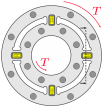
\includegraphics[height=0.4\textheight]{fig/lec01/Torque_shaft_cross_section.pdf}
            \caption{Torque flange cross section (source: \href{https://commons.wikimedia.org/wiki/File:Torque_Flange.gif}{Wikimedia Commons}, M.~Laible, \href{https://creativecommons.org/licenses/by-sa/2.5/deed.en}{CC BY-SA 2.5})}
        \end{subfigure}
        \caption{Torque measurement (via torque-induced strain sensors)}
        \label{fig:torque_sensor}
    \end{figure}
    \vspace{-0.5cm}
    \begin{varblock}{}
        Due to costs, weight and volume of torque sensors, drive systems typically rely on indirect model-based torque estimation. In practice, only test benches and special application needs warrant direct torque measurement.
    \end{varblock}
\end{frame}
